\documentclass[11pt,oneside,a4paper,notitlepage]{article}


\usepackage{float}
\usepackage{amsmath, amsfonts, amssymb}
\usepackage{xcolor}
\usepackage{xfrac}
\usepackage{tikz}
\usetikzlibrary{shapes,arrows}

\usepackage{hyperref}

\usepackage{pgfplots}

\usepackage{pdflscape}



\newcommand{\vect}[1]{\mathbf{#1}}
\setcounter{MaxMatrixCols}{20}

\addtolength{\hoffset}{-15mm} \addtolength{\textwidth}{30mm}
\addtolength{\voffset}{-15mm} \addtolength{\textheight}{30mm}

% change default rm font family 
%\renewcommand*\rmdefault{ppl}


\linespread{1.3} % Increase line spacing by 50%


\usepackage{natbib}

\usepackage{CJKutf8}


\begin{document}
\begin{CJK}{UTF8}{gbsn}
\begin{center} 
\begin{Large}
% title
量化模型总结
\end{Large}
\\
\vspace{4mm}
%author
\vspace{0.5em}
-- Created: April 24, 2024 \\
-- Last Modified: \today
\end{center}
\vspace{2em}
\textbf{Abstract}: 介绍我了解的量化交易中使用的时序模型、因子模型和机器学习模型。 

\section{什么是模型}
模型是用来表示一个关系的东西,关系不一定是因果关系,但我们仍用自变量$\vect x$和因变量$y$这样的名字。所以模型就可以写为 

\begin{equation}
  f(\vect x): \vect x\mapsto y
\end{equation}

如果我们对资产收益率$r$建模,那么$y = r$, $\vect x$表示影响资产收益率的因素。

通过选取不同的$f$的形式,能得到下面几种模型: 时间序列模型、因子模型、机器学习模型。

\subsection{时间序列模型}
时间序列模型的$\vect x$选择收益率的历史序列 $\vect x = \left[r_{t-1}, \ldots, r_{t-K} \right]$, $y = r_t$。
这种模型的假设是收益率受一些未知随机因素影响(MA),并且受自己历史值的影响(AR)。 最常用的时间序列模型是ARIMA模型。中间的I是通过差分把不平稳的序列变平稳。
\subsubsection{ARIMA模型}
对一个时间序列进行ARIMA(p,d,q)模型建模步骤如下:
\begin{enumerate}
\item 序列的平稳性检验。如果不平稳,需要利用一次或多次差分将其转化为平稳序列。如果怎么差分都不平稳,放弃ARIMA模型。
\item 白噪声检验。如果序列是白噪声,可以终止对该序列的分析。啥模型都不管用。
\item 对于平稳非白噪声序列,可以用ARIMA(p,d,q)模型(加入I主要是将非平稳序列转换为平稳序列,d是差分阶数)。
\item 模型定阶,把p,d,q算出来。
\item 参数估计, 包括系数检验和拟合优度检验
\item 残差序列的白噪声检验。
\item 预测。
\end{enumerate}

  参考:
  \begin{enumerate}
 \item  \href{https://yuchen112358.github.io/2016/10/09/ARIMA/}{ARIMA模型建模的具体过程}
 \item  \href{https://blog.csdn.net/weixin\_45590329/article/details/112818196}{使用python的statsmodels模块拟合ARIMA模型}
  \end{enumerate}
\subsubsection{ARCH系列模型}
ARIMA模型主要在刻画收益率的均值,它假设扰动项为白噪声序列,实际上收益率的方差存在聚集效应。条件异方差模型就是在均值建模的基础上,再增加一个收益率的方差随时间变化的模型。这可以更精确刻画收益率的条件分布。

\subsection{因子模型}
因子模型假设不同资产的收益率由共同的因子影响,并将这些共同因子的收益率做为自变量。 
\subsubsection{CAPM}
最简单的因子模型是CAPM模型,它只有一个市场因子,其收益率记为$r_M$,则CAPM单因子模型可写为
$$r_t = \beta r_{M,t} + \epsilon_t $$

为简单起见,上面的$r_t$和$r_{M,t}$分别表示减去无风险利率$r_f$之后的值,表示超额收益 risk premium,下标$t$表示时间,资产下标$i$省略,如果不特别说明,$r_t$表示某个资产在$t$时刻的超额收益。

收益率使用百分比收益率,主要原因是百分比收益率可以做加权求和,这样因子模型就能用到资产组合上来。

当我们对式子左侧求期望,就可以得到资产的预期收益率,同样,对于N个资产组成的资产组合,我们可以求他们的协方差。由预期收益率和协方差矩阵,就可以通过mean-variance optimisation来求资产组合的最优权重。


\subsubsection{Fama-French三因子模型}
再复杂点是Fama和French于1993年提出来的三因子模型。

除了市场因子之外,Fama-French三因子模型还引入了大小Size和价值Value两个因子。Size由公司的BM boot to market ratio反映,价值用市值market value来反映,BM和MV明显是不独立的, 为了保证因子的独立,在构造因子时使用了多重排序法,也就出来的经典的SMB和HML。

但是SMB和HML并不是因子收益率,所以要通过Fama-McBeth回归得到以因子收益率为自变量的回归方程。
$$r_t = \beta_M r_{M,t} + \beta_{SMB}r_{SMB,t} + \beta_{HML} r_{HML,t} + \epsilon_t$$

\subsubsection{Barra 风险模型}
与Fama-French模型用来解释资产收益率不同,风险模型比如MSCI Barra 的目标是更准确地估计资产的协方差矩阵。虽然收益模型和风险模型可以用同样的因子,但貌似预期收益和风险确实受不同因子的影响。
Barra的CNE5模型有1个国家因子,P个行业因子,Q个风格因子。具体写为
  $$r_t = 1\lambda_{C,t} + \sum_i^P{\beta_{I_i}\lambda_{I_i, t}} + \sum_i^Q{\beta_{S,i}\lambda_{S_i, t}} +\epsilon_t $$

式中$\lambda_{C,t}$是t时刻国家因子的收益率,经推导,国家因子收益率基本等于市场组合的超额收益,即前面模型中的市场因子。但是CNE5强制所有资产在国家因子上的暴露为1,这是不同的点。
另外Barra模型的因子收益率计算方法和Fama-MacBeth方法有点区别,它直接使用公司特征作为因子暴露的原始值,而不是时序回归系数。


Barra CNE5S, CNE6模型的数据来源有
\begin{enumerate}
\item 股票和指数的日行情数据,包含turnover rate, amount, return, close, circ mv, total mv, index return 
\item 三大财务报表(季度数据):利润表income, 资产负债表balancesheet、现金流表cashflow
\item 公司主要财务分析指标新会计准则(季度数据),根据报告期公布的财务科目数据衍生而来的指标,tushare 叫fina indicator, akshare里没找到,不清楚是不是财报必须的
\item 一级行业数据,如果某支股票换行业的话,是否要考虑?
\item 分析师预测数据,有可能来自wind万得,无法获取。
\end{enumerate}

Barra因子原始值的计算,核心是数据频率的转换,尤其把季频数据转为日或者月频时,要考虑是使用上一年的数据,还是上一季度的数据,比如Market leverage MLEV因子中的PE和LD在CNE5S中使用的是most recent quarter, 在CNE6中使用的是上一财年last fiscal year的数据。 有些要用ttm值的,还需要计算ttm。

数据的频率转换完成之后,按公式计算即可。

如果使用python的pandas,DataFrame的格式为,每行为一天,每列为一支股票,天为索引,如下所示
\begin{verbatim}
             600221.SH  601006.SH  601288.SH  603127.SH  603206.SH
trade_date                                                       
2022-04-29   0.000000  -0.020588   0.000000   0.085789        NaN
2022-05-05  -0.033520  -0.010511   0.006536  -0.035183        NaN
2022-05-06  -0.028902  -0.013657  -0.009740  -0.029902   0.439780
2022-05-09   0.005952   0.012308   0.006557   0.003652   0.099904
2022-05-10  -0.005917  -0.009119   0.006515  -0.003959   0.099957
\end{verbatim}

具体的计算使用的是github上开源的代码 
\href{https://github.com/ShiliangZhang-nku/Barra_CNE6}{ShiliangZhang-nku Barra CNE6}

我的数据来自数据库,数据采集部分的代码修改自\href{https://github.com/phonegapX/alphasickle}{phonegapX alphasickle}.

需要做一个适配层来适配这两份代码,最终数据采集和因子生成两部分的代码结构如图\ref{fig:cne6}。
\begin{figure}
  \centering
  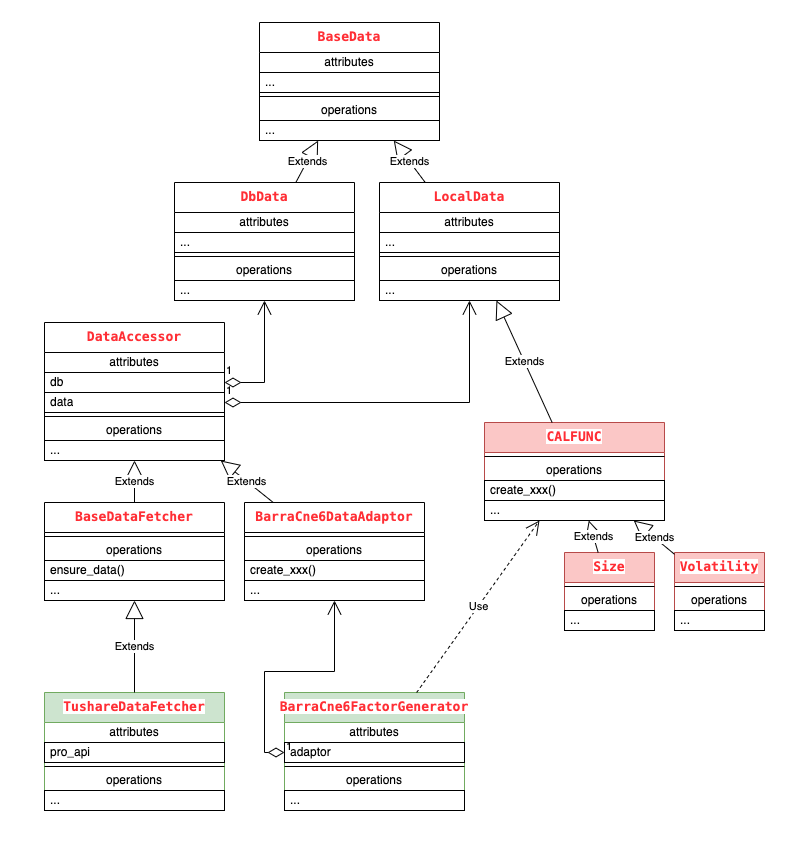
\includegraphics[scale=0.6]{figures/cne6.png}
  \caption{Barra 数据采集与因子计算架构}
  \label{fig:cne6}
\end{figure}





\subsubsection{因子投资组合 factor portfolio}
在使用OLS求解因子模型时,不管是收益模型和风险模型,中间过程存在一个权重矩阵,使得按这个权重对资产配置时,各个组合的收益率互不相交,这些组合被称为因子组合。使用因子组合能够构造特定暴露的资产组合。

\subsubsection{投资组合优化}
有了收益模型和风险模型之后,就可以结合一定的目标函数(比如Markovitz均值方差优化、risk parity等)来求取最优的投资组合。如果风险和收益模型使用不同的因子,一个潜在的问题是优化器会倾向风险模型覆盖不到的那些因子的权重,需要在优化时做特殊考虑。

\subsection{机器学习模型}
这个非常直接,就是找各种特征 $\vect x$, 之后通过数据来训练模型,使其逼近收益率的预测公式 $r_{t+n} = f(\vect x_t)$

\section{未完成的模型}
\begin{enumerate}
    \item 时间序列模型ARIMA
    \item ARCH模型
    \item MSCI CNE5 模型,需要看在风险因子上的暴露
    \item Fama-French 5因子模型
    \item Hou-Xue-Zhang四因子模型
\end{enumerate}


\end{CJK}
\end{document}
